\documentclass[aspectratio=169]{beamer}

\input{src/macros/preamble}
\input{src/macros/sli_aux}

\usepackage{bussproofs}

\begin{document}

% \setLectureBasic{Cyber-Physical Computation}
\setLecture[\\\emph{(slides mainly from Nelma Moreira)}]%
    {3}{CCS: Calculus of Communicating Systems (sequencial)}


\begin{frame}{CCS: \emph{Calculus of Communicating Systems}}

\only<article>{Algebra de processos que permite a especificação se sistemas reactivos (modelados por  sistemas de transição). A combinação de dois processos é um novo processo cujo comportamneto depende dos operandos.}
\only<presentation>{Avô }
Robin Milner: \url{https://en.wikipedia.org/wiki/Robin\_Milner}  (1934-2010)

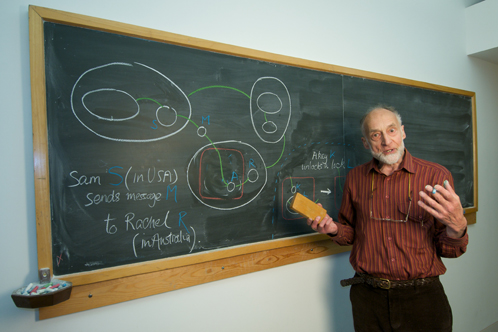
\includegraphics[width=5cm]{src/img/nam/rm.jpg}
\includegraphics[width=4cm]{src/img/nam/cc.png}1989
\end{frame}

\begin{frame}
\only<presentation>{
\frametitle{Robin Milner (1934-2010)}
\begin{description}
	\item[1970s] Edinburgh LCF (Logic of Computable Functions) um dos primeiros demonstradores interactivos de teoremas
	\item[1970s] ML (MetaLanguage): linguagem de programação funcional tipificada (antecessor do OCAML) com inferência de tipos polimórficos (sistema de tipos Hindley-Damas-Milner)
	\item[1980s] Sistemas concorrentes CCS, $\pi$-calculus
	\item [1991] Prémio ACM Turing
	\item [2000s] Bigrafos para computação ubiqua
\end{description}}	
\end{frame}



\begin{frame}

\only<presentation>{\frametitle{CCS:Calculus of Communicating Systems}}

\begin{itemize}[<+->]
	\item o processo mais simples é o que não executa nenhuma ação (deadlock): $0$
\item  Se \alert{$P$} é um processo e \alert{$a$} uma ação, \alert{$a.P$} é um processo que executa \alert{$a$} e depois comporta-se como \alert{$P$}:

\only<2>{\begin{tikzpicture}[>=stealth, shorten >=1pt, auto, node distance=2cm,initial text={}]
\node[st,initial] (S0){a.P};
\node[st][right of =S0] (S1){P};
\path[->](S0) edge  node {\color{red} a}(S1);
\end{tikzpicture}
}
\item  Um fósforo: $strike.light.extinguish.0$\only<3>{\begin{tikzpicture}[>=stealth, shorten >=1pt, auto, node distance=2cm,initial text={}]
\node[st,initial] (S0){};
\node[st][right of =S0] (S1){};
\node[st][right of =S1] (S2){};
\node[st][right of =S2] (S3){};
\path[->](S0) edge  node {\color{red} strike}(S1)
	  (S1) edge   node { \color{red} light }(S2)
         (S2) edge   node { \color{red} extinguish }(S3);
\end{tikzpicture}
}
\item  Uma máquina de vender café: $\text{coin}.\text{coffee}.0$
\only<4>{\begin{tikzpicture}[>=stealth, shorten >=1pt, auto, node distance=2cm,initial text={}]
\node[st, initial] (S0){};
\node[st][right of =S0] (S1){};
\node[st][right of =S1] (S2){};
\path[->](S0) edge  node {\color{red} coin}(S1)
         (S1) edge   node { \color{red}coffee}(S2);
\end{tikzpicture}}

\item Ações internas:  $\tau$
\item Um fósforo que não acende: $strike.\tau.0$
\only<6>{\begin{tikzpicture}[>=stealth, shorten >=1pt, auto, node distance=2cm,initial text={}]
\node[st,initial] (S0){};
\node[st][right of =S0] (S1){};
\node[st][right of =S1] (S2){};
\path[->](S0) edge  node {\color{red} strike}(S1)
	  (S1) edge   node { \color{red} $\tau$ }(S2);
\end{tikzpicture}}

\item Se houver uma escolha: $strike.(light.0 + \tau.0)$
\only<7>{
\begin{tikzpicture}[>=stealth, shorten >=1pt, auto, node distance=2cm,initial text={}]
\node[st,initial] (S0){};
\node[st][right of =S0] (S1){};
\node[st][right of =S1] (S2){};
\path[->](S0) edge  node {\color{red} strike}(S1)
	  (S1) edge [bend left]  node { \color{red} light }(S2)
         (S1) edge  [bend right, swap ] node { \color{red} $\tau$ }(S2);
\end{tikzpicture}
}
\item Dois fósforos em paralelo:  $strike.(light.0 |\tau.0)$ \ 
\only<8>{%\begin{center}
\begin{tikzpicture}[>=stealth, shorten >=2pt, auto, node distance=2cm, initial text={}]
\node[st,  initial] (S0){};
\node[st][ right of =S0] (S1){};
\node[st][right of =S1] (S2){};
\node[st][below left  of =S1] (S3){};
\node[st][right  of =S3] (S4){};

\path[->](S0) edge node { \color{red} $strike$} (S1)
	(S1) edge  node { \color{red} $light$} (S2)
		edge  node [swap] { \color{red} $\tau$} (S3)
	(S2) edge  node { \color{red} $\tau$}(S4)
	(S3) edge  node { \color{red} $light$}(S4);
\end{tikzpicture}}%\end{center}}
\end{itemize}	
\end{frame}

\begin{frame}{Operadores do CCS}
\begin{description}
\item["$.\;$" Prefixo ] a execução de $\alpha.P$ começa com a execução da ação $\alpha\in Act$ e depois comporta-se como $P$.	
\item["$+\;$" Escolha ] O processo $P+Q$ comporta-se como o processo $P$ ou o processo $Q$. É a escolha não determinística.
\item["$|\;$"  Composição Paralela ]
O processo $P| Q$ representa a execução concorrente de $P$ e $Q$ (que progridem independentemente um do outro). 
\end{description}
\end{frame}
\begin{frame}{$CCS_0$ Sequencial sem recursão}
	
Seja $Act$ um conjunto de ações. O conjunto de expressões do $CCS_0$ são dadas pela seguinte gramática
\begin{eqnarray*}
P&::=& 0 \mid P+P \mid \alpha.P
\end{eqnarray*}
onde supomos as seguintes regras de prioridades
\begin{itemize}[<+->]
	\item $P+Q+R$ é $(P+Q)+R$
\item $\alpha.\beta.P$ é $\alpha.(\beta.P)$
\item  $\alpha.P+ Q$ é $(\alpha.P) + Q$
\item e por vezes omitimos o $0$: $\alpha.\beta$ em vez de $\alpha.\beta.0$ 
\item Ex:  $strike.(light.0 + \tau.0) \in CCS_0$
\end{itemize}
\end{frame}

\begin{frame}
	\begin{exem}
	 Quais dos seguintes termos são expressões válidas do $CCS_0$:
	 \begin{enumerate}
	 	\item $0$
	 	\item $a.b.0$\label{ex:2}
	 	\item $(a.b).0$ \label{ex:3}
	 	\item $(a.(b.0))$
		\item $a.b$ \label{ex:4}
		\item  $0.a.b$ \label{ex:6}
		\item $a.(b.0)+0$
		\item $0+0$
		\item $a.(a.0+b.c.0)$
		\item $(a.0+b.c.0).a.0$ \label{ex:9}
	 \end{enumerate}	
	\end{exem}
\only<article>{Os casos \ref{ex:3}, \ref{ex:6} e \ref{ex:9} não são termos do $CCS_0$. O caso \ref{ex:4} é uma abreviatura de \ref{ex:2}}
\end{frame}

\begin{frame}{Book pseuCo.com}
\url{https://book.pseuco.com/\#} Capítulo $CCS_0$.
\end{frame}

\begin{frame}{Semântica do $CCS_0$}
A semântica duma expressão $P$ é um LTS $\bras{P}=(S,\tr,s_0)$. onde:
\begin{itemize}[<+->]
	\item $S=\{Q \mid Q\in CCS_0\}$, i.e.,  as expressões válidas do $CCS_0$ \only<article>{(que tipo de LTS será?)}
\item $s_0=P$
\item $\tr \subseteq  (CCS_0\times Act\times CCS_0)$
\end{itemize}

	\pause 
	
	 \begin{exem}[Fragmento dum LTS para o processo $extinguish.0$]
		\splittwo{0.39}{0.44}{
			~\\[2mm]
			$Act=\{strike,light, extinguish,\tau\}$
			para $\bras{extinguish.0}$
			\\[5mm]
			\url{https://lmf.di.uminho.pt/ccs-caos/?light.extinguish.0}}{
{\small
\begin{center}
\begin{tikzpicture}[>=stealth, shorten >=2.5pt, auto, node distance=2cm, initial text={}]
\node[st,  initial] (S0){$extinguish.0$};
\node[st][below right of =S0] (S1){0};
% \node[st][above right of =S1] (S2){$\tau.0$};
\node[st][below left  of =S0] (S3){$light.extinguish.0$};
% \node[st][below  of =S2] (S4){$\tau.0+\tau.0$};
% \node[st][below right  of =S4, node distance=10mm] (S5){$\tau.0+light.0$};

\path[->](S0) edge node {$extinguish$} (S1)
	(S3) edge [bend left] node {light} (S0);
% (S2) edge  node {$\tau$}(S1)
% (S4) edge  node {$\tau$}(S2)
% (S5) edge [bend right, xshift=0.9,swap]  node {$\tau$}(S2)
	 % edge [bend left,pos=0.8]  node {$light$} (S1);
\end{tikzpicture}\end{center}}
}
\end{exem}
\end{frame}

\begin{frame}
\begin{exem}[Fragmento do LTS acessível  para $extinguish.0$]
		$Act=\{strike,light, extinguish,\tau\}$
para $\bras{extinguish.0}$.   
Mas, pretendemos apenas o fragmento \emph{acessível}, i.e., $Reach(extinguish.0)$: 
{\small\begin{center}
\begin{tikzpicture}[>=stealth, shorten >=2.5pt, auto, node distance=2cm, initial text={}]
\node[st,  initial] (S0){$extinguish.0$};
\node[st][below right of =S0] (S1){0};
\path[->](S0) edge node {$extinguish$} (S1);
\end{tikzpicture}\end{center}}
	\end{exem}
\end{frame}

\begin{frame}{Regras de Inferência - Semântica operacional estrutural}
\begin{itemize}[<+->]
	\item Permitem definir um LTS cujos estados são expressões e existe uma transição $\trans{P}{\alpha}{Q}$ se  esta puder ser demonstrada a partir das regras.
\item Uma regra é da forma $$\frac{P_1 \cdots  P_n}{P}$$
\item $P_1,\ldots,P_n$ são as \alert{Premissas} ou Hipóteses
\item $P$ é a \alert{Conclusão}
\item Significa: se  $P_1,\ldots,P_n$ se verificarem então $P$ também se verifica (pode ser inferido), i.e., os $P_i$ implicam $P$.
\item Se $n=0$ então a $P$ é um \alert{Axioma}
\end{itemize}	
\end{frame}
\begin{frame}{}
%\begin{block}{Regras do $CCS_0$}
%\hrule
%	\begin{eqnarray*}
%	\text{Prefixo}&& \frac{}{\trans{\alpha.P}{\alpha}{P}}\\
%	\text{EscolhaE}&& \frac{\trans{P}{\alpha}{P'}}{\trans{P+Q}{\alpha}{P'}}\\
%\text{EscolhaD}&&\frac{\trans{Q}{\alpha}{Q'}}{\trans{P+Q}{\alpha}{Q'}}
%	\end{eqnarray*}
%\hrule
%\end{block}

\begin{block}{Regras do $CCS_0$}
% \hrule
	\begin{prooftree}
	\LeftLabel{Prefixo} \AxiomC{}
\UnaryInfC{$\trans{\alpha.P}{\alpha}{P}$}
\end{prooftree}
\begin{prooftree}
	\LeftLabel{EscolhaE} \AxiomC{$\trans{P}{\alpha}{P'}$}
\UnaryInfC{$\trans{P+Q}{\alpha}{P'}$}
\end{prooftree}
\begin{prooftree}
	\LeftLabel{EscolhaD} \AxiomC{$\trans{Q}{\alpha}{Q'}$}
\UnaryInfC{$\trans{P+Q}{\alpha}{Q'}$}
\end{prooftree}
% \hrule
\end{block}
\end{frame}

\begin{frame}{Exemplo}
	$$\bras{\text{coin}.\text{coffee}.0}$$
\only<2->{
\
\begin{prooftree}
\RightLabel{Prefixo}\AxiomC{}
 \UnaryInfC{$\trans{coin.coffee.0}{coin}{coffee.0}$}
\end{prooftree}

}
\only<3->{
\begin{prooftree}
\RightLabel{Prefixo}
 \AxiomC{}\UnaryInfC{$\trans{coffee.0}{coffee}{0}$}	
 \end{prooftree}
}

\only<4>{\centerline{\begin{tikzpicture}[>=stealth, shorten >=3pt, auto, node distance=3cm,initial text={}]
\node[st, initial] (S0){$coin.coffee.0$};
\node[st][right of =S0] (S1){$coffee.0$};
\node[st][right of =S1] (S2){$0$};
\path[->](S0) edge  node {coin}(S1)
         (S1) edge   node {coffee}(S2);
\end{tikzpicture}}}
\medskip

\only<5>{\centerline{\begin{tikzpicture}[>=stealth, shorten >=1pt, auto, node distance=2cm,initial text={}]
\node[st, initial] (S0){};
\node[st][right of =S0] (S1){};
\node[st][right of =S1] (S2){};
\path[->](S0) edge  node {\color{red} coin}(S1)
         (S1) edge   node { \color{red}coffee}(S2);
\end{tikzpicture}}}
\medskip

\only<presentation>{

{\flushbottom\hrule
Regras:
$\begin{array}{lrlrlr}
\text{Prefixo}& \frac{}{\trans{\alpha.P}{\alpha}{P}}&
	\text{EscolhaE}& \frac{\trans{P}{\alpha}{P'}}{\trans{P+Q}{\alpha}{P'}}&
\text{EscolhaD}&\frac{\trans{Q}{\alpha}{Q'}}{\trans{P+Q}{\alpha}{Q'}}
\end{array}$}
}

\end{frame}


\begin{frame}{Exemplo}
\only<1->{$$\bras{(a.0+0)+b.(0+0)}$$}
\only<2->{
\begin{flushleft}
\begin{prooftree}
\RightLabel{Prefixo}\AxiomC{}
 \UnaryInfC{$\trans{a.0}{a}{0}$}\RightLabel{EscolhaE}
\UnaryInfC{$\trans{a.0+0}{a}{0}$}\RightLabel{EscolhaE}
 \UnaryInfC{$\trans{(a.0+0)+b.(0+0)}{a}{0}$}
\end{prooftree}
\end{flushleft}
}
\only<3->{
\begin{flushright}
\begin{prooftree}
\RightLabel{Prefixo}
 \AxiomC{$\trans{b.(0+0)}{b}{0+0}$}	\RightLabel{EscolhaD}
 \UnaryInfC{$\trans{(a.0+0)+b.(0+0)}{b}{0+0}$}
\end{prooftree}
\end{flushright}}

\only<4>{{\small
\begin{tikzpicture}[>=stealth, shorten >=2.5pt, auto, node distance=1.5cm, initial text={}]
\node[state,rectangle, rounded corners=7pt,  inner sep=4pt, minimum size=5pt,  initial] (S0){$(a.0+0)+b.(0+0)$};
\node[state,rectangle, rounded corners=7pt,  inner sep=4pt, minimum size=5pt][below right of =S0] (S1){0};
\node[state,rectangle, rounded corners=7pt,  inner sep=4pt, minimum size=5pt][below =0.8 of S0] (S2){$0+0$};
\path[->](S0) edge node {$a$} (S1)
	edge  node {$b$} (S2);
\end{tikzpicture}}
}

\only<presentation>{

\only<1-3>
{\flushbottom\hrule
Regras:
$\begin{array}{lrlrlr}
\text{Prefixo}& \frac{}{\trans{\alpha.P}{\alpha}{P}}&
	\text{EscolhaE}& \frac{\trans{P}{\alpha}{P'}}{\trans{P+Q}{\alpha}{P'}}&
\text{EscolhaD}&\frac{\trans{Q}{\alpha}{Q'}}{\trans{P+Q}{\alpha}{Q'}}
\end{array}$}
}

\only<article>{
	\begin{exerc}
	Determina:
	\begin{enumerate}
		\item $\bras{light.(burn.extinguish.0+smolder.0)}$
		\item $\bras{a.(b.0+a.(0+0)+0)+b.0+a.(0+0)}$
	\end{enumerate}	
	\end{exerc}
}
\end{frame}


\begin{frame}
\frametitle{Semântica do $CCS_0$ (II)}

A relação $\tr$ é a menor tal que, para todo $\alpha\in Act$ e $P,Q\in CCS_0$,
\begin{itemize}
	\item  $(\alpha.P,\alpha,P)\in \tr$
\item    $(P+Q,\alpha,P')\in \tr)$ se $(P,\alpha,P')\in \tr$
\item    $(P+Q,\alpha,Q')\in \tr)$ se $(Q,\alpha,Q')\in \tr$
\item nada mais está em $\tr$
\end{itemize}

\only<presentation>{\bigskip\bigskip

{\flushbottom\hrule
Regras:

$\begin{array}{lrlrlr}
\text{Prefixo}& \frac{}{\trans{\alpha.P}{\alpha}{P}}&
	\text{EscolhaE}& \frac{\trans{P}{\alpha}{P'}}{\trans{P+Q}{\alpha}{P'}}&
\text{EscolhaD}&\frac{\trans{Q}{\alpha}{Q'}}{\trans{P+Q}{\alpha}{Q'}}
\end{array}$}
	}
\end{frame}


\begin{frame}
%{Semântica do $CCS_0$ (II)}
O conjunto de todos os LTSs sobre expressões do $CCS_0$ é 
$$LTS_0 = \{(CCS_0,T,P)\mid T\subseteq (CCS_0\times Act\times CCS_0), P\in CCS_0\}$$
A semântica das expressões do $CCS_0$ é então $$\bras{\_}: CCS_0\fun LTS_0$$ tal que $$\bras{P}=(CCS_0,\tr,P)$$ com $\tr$ definida anteriormente.
\end{frame}
\begin{frame}
\begin{itemize}
	\item Contudo apenas interessa  um fragmento de $\bras{P}$
\item Só interessam estados atingíveis de $P$
\item Só interessam as acções dos estados atingíveis
\item  Não interessam os nomes dos estados atingíveis
\item Por exemplo $\alpha.0+0$ e $0+\alpha.0$ não têm o mesmo LTS  (verifica) mas são \alert{isomorfos}.
\end{itemize}
\end{frame}



\begin{frame}{Isomorfismo}
	Dois LTS $TS=(S,\tr,s_0)$ and $TS'=(S',\tr',s_0')$ são isomorfos, $TS\sim TS'$,  se existe uma bijeção $f$ com
$$f: Reach(TS) \fun Reach(TS')$$
com
\begin{itemize}
	\item $f(s_0)=s_0'$
\item para todos os $s_1,s_2\in Reach(TS)$ e para toda $\alpha \in Act$ 
\begin{eqnarray*}
	\trans{s_1}{\alpha}{s_2}& sse &	\trans{f(s_1)}{\alpha}{'f(s_2)}
\end{eqnarray*}
\item Dois LTSs isomorfos são indistinguíveis para um observador.
\end{itemize} 

\end{frame}

\only<article>{
\begin{frame}
	\begin{exerc}
	Mostrar que o isomorfismo de LTSs é uma relação de equivalência.	
	\end{exerc}
\begin{exerc}
	Mostrar que um LTS que é finitamente ramificado e tem um número finito de estados é isomorfo a um LTS finito por estados.
	\end{exerc}
\begin{exerc}
Mostra que dado um LTS finito $TS$  (acíclico) existe uma expressão $P$ do $CCS_0$ 	tal que $TS=\bras{P}$.
\end{exerc}

\end{frame}
}


\begin{frame}{Definições Recursivas em CCS}

\begin{itemize}[<+->]
\item  Como representar o seguinte LTS (máquina de café):
\only<1>{
\begin{center}
\begin{tikzpicture}[>=stealth, shorten >=1pt, auto, node distance=3cm,initial text={}]
\node[st] (S0){};
\node[st][right of =S0] (S1){};
\path[->](S0) edge [bend left] node {\color{red} coin}(S1)
         (S1) edge  [bend left] node { \color{red} coffee}(S0);
\end{tikzpicture}
\end{center}
}
	\item  Usando \alert{nomes} para sub-expressões e  que podem ser usadas em expressões.
\item Em vez de $strike.(light.0  + \tau.0)$
\begin{eqnarray*}
	Match &:= & strike.MatchOneZeroLight\\
MatchOneZeroLight &:= & light.0 + \tau.0
\end{eqnarray*}
\only<3>{
\begin{tikzpicture}[>=stealth, shorten >=1pt, auto, node distance=2cm,initial text={}]
\node[st,initial] (S0){};
\node[st][right of =S0] (S1){};
\node[st][right of =S1] (S2){};
\path[->](S0) edge  node {\color{red} strike}(S1)
	  (S1) edge [bend left]  node { \color{red} light }(S2)
         (S1) edge  [bend right, swap ] node { \color{red} $\tau$ }(S2);
\end{tikzpicture}
}
\item sendo que agora podemos representar repetição (iteração)
\begin{eqnarray*}
	Match &:= & strike.MatchOnFire\\
MatchOnFire &:= & light.MatchOnFire + extinguish.0
\end{eqnarray*}
\only<4>{\begin{tikzpicture}[>=stealth, shorten >=2.5pt, auto, node distance=3.5cm, initial text={}]
\node[state, rectangle, rounded corners=7pt,  inner sep=4pt, minimum size=5pt,  initial] (S0){$Match$};
\node[state, rectangle, rounded corners=7pt,  inner sep=4pt, minimum size=5pt][right of =S0] (S1){$MatchOnFire$};
\node[state, rectangle, rounded corners=7pt,  inner sep=4pt, minimum size=5pt][right of =S1] (S2){$0$};
\path[->](S0) edge node {$strike$} (S1)
	(S1) edge  node {$extinguish$} (S2)
			edge [loop below] node  {$light$} ();
\end{tikzpicture}
}
\item \alert{Convenção}: nomes  (de sub-expressões) começam por uma letra maiúscula e ações por minúscula. Também são chamadas de \emph{constantes} ou \emph{variáveis}. 
\end{itemize}

	\end{frame}
	
	\begin{frame}{$CCS_0^\omega$ : Sequencial com iteração}
	Seja $Act$ um conjunto de ações e $Var$ um conjunto de nomes (variáveis). As expressões do $CCS_0^\omega$ são
\begin{eqnarray*}
P&::=& 0 \mid X \mid P+P \mid \alpha.P
\end{eqnarray*}
onde 
\begin{itemize}
	\item 
$
\alpha \in Act$, 
\item $X\in Var$ e 
\item uma função  parcial de $Var \fun CCS_0^\omega$, \alert{$\Gamma$}, que pode ser representada por um conjunto   de equações da forma $X:=P$ ou representada por pares $(X,P)$
$$\Gamma=\{(X_1,P_1),\ldots, (X_n,P_n)\}$$
onde\\[-10mm]
\begin{align*}
	\Gamma(X_i)=P_i && \text{ou apenas} &&X_i:= P_i, && 1\leq i\leq n. \end{align*}
A função $\Gamma$ representa um \emph{ambiente}.
\end{itemize}
\end{frame}

\begin{frame}
\begin{exem}\ 
\begin{enumerate}[<+->]
	\item $X:=a.b.X$ então temos $\Gamma=\{(X,a.b.X)\}$
\item  Se \begin{eqnarray*}
 X&:=& a.b.Y\\
Y&:= & b.Z +a.Y\\
	Z&:=& a.Y
 \end{eqnarray*}
temos $\Gamma=\{(X,a.b.Y),(Y,b.Z+a.Y),(Z,a.Y)\}$.
\end{enumerate}
\end{exem}
\end{frame}

\begin{frame} \frametitle{Regra da Recurção}

\begin{prooftree}
	\LeftLabel{Rec} \AxiomC{$\trans{P}{\alpha}{P'}$}
\AxiomC{$\Gamma(X)=P$}
\BinaryInfC{$\trans{X}{\alpha}{P'}$}
\end{prooftree}

\only<2->{\begin{exem}
 Determinar $\bras{X}_\Gamma$ com $\Gamma=\{(X,a.b.X)\}$, i.e., temos a equação
 $X:=a.b.X$
\begin{columns}
\begin{column}{0.7\textwidth}
\begin{prooftree}
\LeftLabel{Prefixo}\AxiomC{}
	\UnaryInfC{$\trans{a.b.X}{a}{b.X}$}
\AxiomC{$\Gamma(X)=a.b.X$}
\LeftLabel{Rec} \BinaryInfC{$\trans{X}{a}{b.X}$}
\end{prooftree}

\end{column}	
\begin{column}{0.3\textwidth}
\begin{prooftree}
\AxiomC{}
\LeftLabel{Prefixo} \UnaryInfC{$\trans{b.X}{b}{X}$}
\end{prooftree}
\end{column}
\end{columns}
\only<3->{\centerline{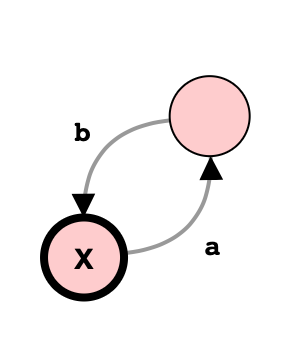
\includegraphics[width=2cm]{src/img/nam/rec00lts}
O segundo estado é etiquetado por $b.X$}}
\end{exem}}
\end{frame}

	

\begin{frame}{Semântica do $CCS_0^\omega$ }
\begin{block}{Regras do $CCS_0^\omega$}
\hrule
	\begin{prooftree}
	\LeftLabel{Prefixo} \AxiomC{}
\UnaryInfC{$\trans{\alpha.P}{\alpha}{P}$}
\end{prooftree}
\begin{prooftree}
	\LeftLabel{EscolhaE} \AxiomC{$\trans{P}{\alpha}{P'}$}
\UnaryInfC{$\trans{P+Q}{\alpha}{P'}$}
\end{prooftree}
\begin{prooftree}
	\LeftLabel{EscolhaD} \AxiomC{$\trans{Q}{\alpha}{Q'}$}
\UnaryInfC{$\trans{P+Q}{\alpha}{Q'}$}
\end{prooftree}
\begin{prooftree}
	\LeftLabel{Rec} \AxiomC{$\trans{P}{\alpha}{P'}$}
\AxiomC{$\Gamma(X)=P$}
\BinaryInfC{$\trans{X}{\alpha}{P'}$}
\end{prooftree}
\hrule
\end{block}

\end{frame}

\begin{frame}{Semântica do $CCS_0^\omega$ }
	A relação $\tr_\Gamma$ é a menor tal que, para todo $\alpha\in Act$ e $P,Q\in CCS_0^\omega$,
\begin{itemize}
	\item  $(\alpha.P,\alpha,P)\in \tr_\Gamma$
\item    $(P+Q,\alpha,P')\in \tr_\Gamma)$ se $(P,\alpha,P')\in \tr_\Gamma)$
\item    $(P+Q,\alpha,Q')\in \tr_\Gamma)$ se $(Q,\alpha,Q')\in \tr_\Gamma)$
\item\alert{ $(X,\alpha,P')\in\tr_\Gamma$ se $\Gamma(X)=P$ e $(P,\alpha,P')\in \tr_\Gamma $}
\item nada mais está em $\tr_\Gamma$
\end{itemize}
\pause
\begin{block}{Regra prática}
Tentar aplicar as regras a um $P$ até encontrar uma nova transição $\trans{P}{\alpha}{P'}$. E repetir para $P'$ caso não fosse conhecido  ele ou o seu comportamento.	
\end{block}

\end{frame}


\begin{frame}
\begin{exem}
Determinar $\bras{M}_\Gamma$ com $\Gamma=\{(M, coin.coffee.M)\}$ ou seja $$M:=coin.coffee.M$$
\only<2->{
	\begin{prooftree}
\LeftLabel{Prefixo}\AxiomC{}
	\UnaryInfC{$\trans{coin.coffee.M}{coin}{coffee.M}$}
\AxiomC{$\Gamma(M)=coin.coffee.M$}
\LeftLabel{Rec} \BinaryInfC{$\trans{M}{coin}{coffee.M}$}
\end{prooftree}}
\only<3->{\begin{prooftree}
\AxiomC{}
\LeftLabel{Prefixo} \UnaryInfC{$\trans{coffee.M}{coffee}{M}$}
\end{prooftree}}
\only<4->{
\begin{center}
\begin{tikzpicture}[>=stealth, shorten >=1pt, auto, node distance=3cm,initial text={}]
\node[st] (S0){$M$};
\node[st][right of =S0] (S1){$coffee.M$};
\path[->](S0) edge [bend left] node {coin}(S1)
         (S1) edge  [bend left] node { coffee}(S0);
\end{tikzpicture}
\end{center}}
\end{exem}
	

\only<article>{
\begin{exerc} Determinar
$\bras{Y}_\Gamma$ com $\Gamma=\{(X,a.b.Y),(Y,b.Z+a.Y),(Z,a.Y)\}$, i.e.,
$X:=a.b.Y$, $Y:=b.Z+a.Y$ e $Z:=a.Y$
\centerline{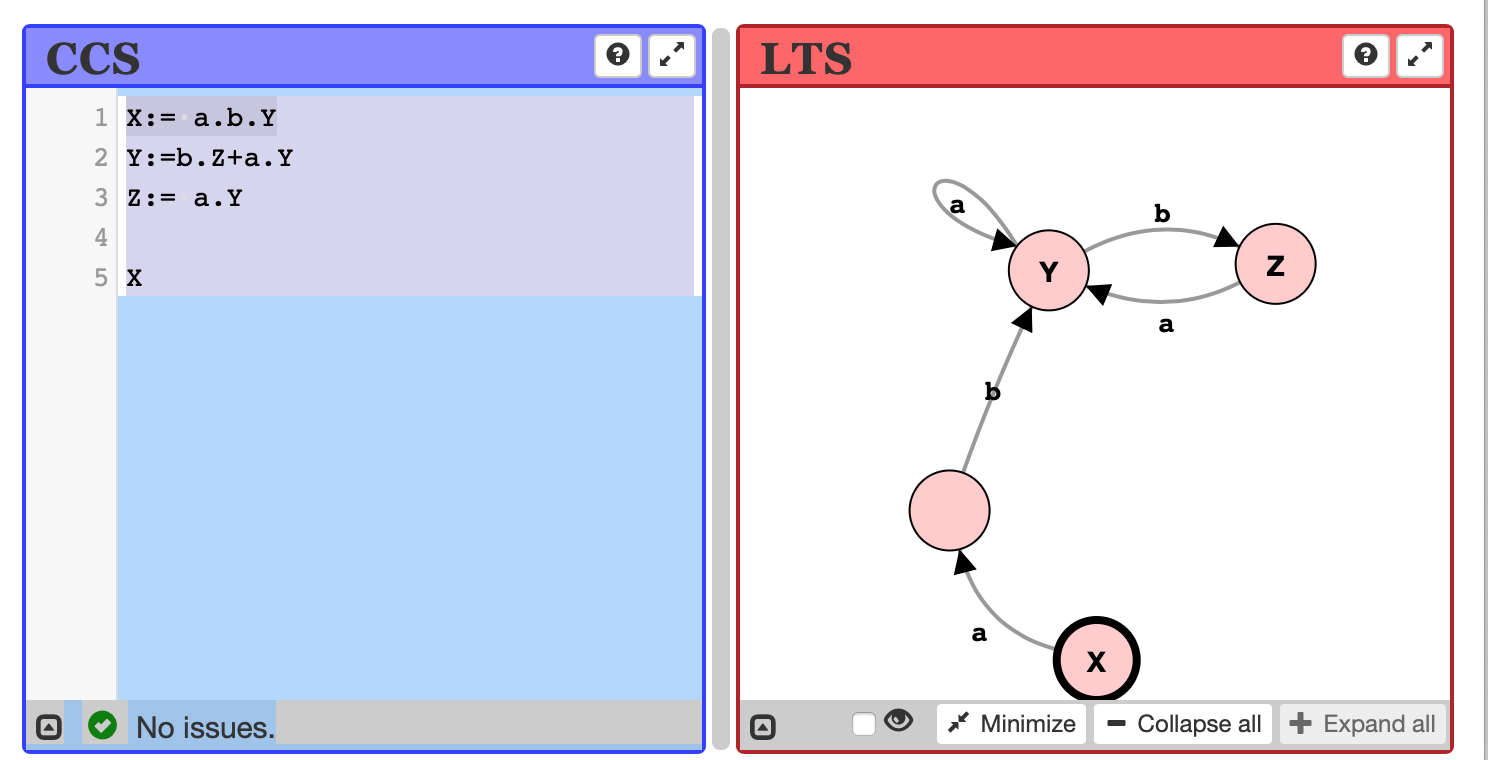
\includegraphics[width=8cm]{src/img/nam/rec0lts}}
	Determinar formalmente $\bras{Y}_\Gamma$. 
\end{exerc}}
	
\end{frame}

\begin{frame}<beamer:0>
\begin{exem}
$\bras{X}_\Gamma$ e $\Gamma=\{(X,0+Y),(Y,a.X)\}$ ( 
$X:=0+Y$ e $Y:=a.X$)
\begin{prooftree}
\AxiomC{}
\LeftLabel{Prefixo} \UnaryInfC{$\trans{a.X}{a}{X}$}
\AxiomC{$\Gamma(Y)=a.X$}
\LeftLabel{Rec} \BinaryInfC{$\trans{Y}{a}{X}$}
\LeftLabel{EscolhaD} \UnaryInfC{$\trans{0+Y}{a}{X}$}
\AxiomC{$\Gamma(X)=0+Y$}
\LeftLabel{Rec} \BinaryInfC{$\trans{X}{a}{X}$}
\end{prooftree}
 Desenha o LTS $\bras{X}_\Gamma$ e $\bras{Y}_\Gamma$  
	\end{exem}
\end{frame}




\begin{frame}{Mais Exemplos}
Como calcular:
\begin{itemize}
	\item $\bras{X}_\Gamma$ e $\Gamma=\{(X,X)\}$ 
\item $\bras{X}_\Gamma$ e $\Gamma=\{(X,X+a.0)\}$ 
\item $\bras{X_0}_\Gamma$ e $\Gamma=\{(X_i,a.X_{i+1})\mid i\geq 1\}$ 
\end{itemize}

\pause
\end{frame}
\only<article>{
\begin{frame}
\begin{exerc}
	Dado 
	$$BurningMatch:=burn.BurningMatch+extinguish.0$$
	
	calcula o LTS do seguinte processo $strike.(BurningMatch+smolder.0$, i.e.,
	$\bras{strike.(BurningMatch+smolder.0)}$.
	
	Usa também o pseuco.com.
	
	\end{exerc}

\end{frame}
}
\begin{frame}
	\begin{exerc}
	Tenta calcular $\bras{X}$ com $\Gamma=(X, X+a.X)$
	\end{exerc}

Se se usar a regra EscolhaE podemos ter árvores de dedução infinitas que não levam a novas transições. Assim iremos evitar esse tipo de expressão (embora sintaticamente correctas).
\end{frame}

\begin{frame}{Expressões guardadas}
\begin{itemize}[<+->]
	\item Uma variável $X$ é \alert{guardada} na expressão $P$ se cada ocorrência de $X$ em $P$ ocorre numa expressão $\alpha.Q$
\item caso contrário \alert{não é guardada}
\item Uma expressão é guardada se todas as suas  variáveis são guardadas
\item caso contrário \alert{não é guardada}
\item Ex. não guardadas: $X$, $a.0+X$, $\tau.X+Y$, $a.X+Y$
\item  Ex. guardadas: $a.X$, $a.(X+Y)$, $\tau.X +a.Y$, $a.(X+b.Y)$
\item Se todas as imagens de um ambiente $\Gamma$  (i.e. $\Gamma(X)$) são guardadas dizemos que $\Gamma$ é \emph{guardado}.
\item Se $P\in CCS_0^\omega$ é  guardada  e os valores de $\Gamma$ são guardados, é possível calcular $\bras{P}_\Gamma$ pela regra prática, isto é o processo termina.
\item No pseuco.com só há expressões guardadas
\end{itemize}
\end{frame}

\begin{frame}<beamer:0>
\frametitle{Semântica do $CCS$ Sequencial (III)}
$$LTS_0^\omega = \{(CCS_0^\omega,T,P)\mid T\subseteq (CCS_0^\omega\times Act\times CCS_0^\omega, P\in CCS_0^\omega\}$$
Conjunto de todos os LTS sobre expressões do $CCS_0^\omega$ com um conjunto de variáveis $Var$. A semântica das expressões do $CCS_0^\omega$ é então $$\bras{\_}: (Var\fun CCS_0^\omega) \fun CCS_0^\omega \fun LTS_0^\omega$$ tal que $$\bras{P}_\Gamma=(CCS_0^\omega,\tr_\Gamma,P)$$ com $\tr_\Gamma$ definida anteriormente e $\Gamma\in Var\fun CCS_0^\omega$.
\end{frame}
\begin{frame}<beamer:0>
	\begin{exerc}
		Mostrar que para cada LTS estados-finito existe uma expressão $P\in CCS_0^\omega$ tal que $TS \sim \bras{P}_\Gamma$.
	\end{exerc}

\end{frame}

\begin{frame}
	\begin{exem}
		
	\end{exem}

\end{frame}

\begin{frame}
\begin{exem}{Exemplos de $1-Buffer$ (de uma posição)}

Considera as  equações de $\Gamma$ seguintes.
\begin{enumerate}
\item Calcula $\bras{Buffer}_\Gamma$.
\begin{eqnarray*}
	Buffer &:=& put?. get?.Buffer
\end{eqnarray*}

\item Calcula $\bras{put?.BufferM}_\Gamma$.
\begin{eqnarray*}
	BufferM &:=& put?. get?.BufferM + get?.put?.BufferM
\end{eqnarray*}
\item Calcula $\bras{Buffer0}_\Gamma$.
\begin{eqnarray*}
	Buffer0 &:=& put?.Buffer1 \\
	Buffer1 &:=& get?.Buffer2 + get?.Buffer0\\
	Buffer2 &:=& get?.Buffer1\\
\end{eqnarray*}

\end{enumerate}
\end{exem}
\end{frame}

\begin{frame}{PseuCo.com \& CCS-Caos}
\url{https://pseuco.com/}{}

\bigskip

\url{https://lmf.di.uminho.pt/ccs-caos/}{}

\end{frame}


\end{document}